\section{Introduction}
%According to the report in the first quarter of 2016, Android devices accounted for a market share of 76.4\%\cite{01}. Android apps generate lots of revenue which is increasing every years. While many apps can be repackaged and cloned easily using off-the-shelf tools like apktool\cite{33} or IDApro\cite{34}, in order to obtain privacy of users, extort and deceive the money of users. This significantly threaten the fast growing mobile app market, which is estimated to value at \$5.5billions in 2015 and will reach \$8.9billions in 2018\cite{02}. Thus, it is necessary and urgent to propose a protection method for Android applications.

Unauthorized code reverse engineering is a major concern for Android
application developers. This technique is widely used by adversaries to
perform various attacks, including removing copyright protection to obtain an
illegal copy of the software, taking out advertisement from the app, or
injecting malicious code into the program. By making the program harder to be
traced and analyzed, code obfuscation is viable means to
protect applications from unauthorized code modification.


A number of code obfuscation approaches have been proposed to protect
applications against code reverse engineering~\cite{06,07,08,09}. Most of the
prior work perform code obfuscation on high-level programming languages such
as java and require access to the program source code. However, this
requirement has two major drawbacks: (1) source code level code obfuscation
provides limited protection as the obfuscated code can removed or
optimized out by the compiler; (2) many developers are not willing to disclose
their source code.  As such, a code
protection technique performing on the compiled bytecodes with stronger protection is highly attractive.


The first effort in this direction is SMOG~\cite{10} that performs code
obfuscation by permuting the instruction opcodes from the compiled Dex
bytecode\footnote{Dalvik Executable format (DEX) is the executable binary format for Android
applications. It was originally designed for the Dalvik VM, which is then
remained to be used by the latest Android runtime (ART).}. The permutated opcodes are then
interpreted at runtime through a modified VM interpreter. While promising,
there is a significant shortcoming of this approach. Because the permutation
is statically determined and hard-coded, SMOG can only resist static but not
dynamic analysis where an attacker can discover the mapping of opcodes through
profiling the application to trace the permutation. Therefore, a technique to
protect the application against both static and dynamic analysis is needed.


%Majority of security solutions have been designed and deployed primarily focusing on the client side interests. Firewalls\cite{28,29}, Intrusion Detection \& Prevention Systems (IDPS)\cite{30,31}, antivirus\cite{32}, digitally signed software, etc. are examples of security applications that provide software protection at the user end but do not degend against the software vulnerabilities exploited by attackers and reverse engineers. Therefore, it is imperative to propose a method to increase the difficulty of reverse engineering. One of the techniques used against reverse engineering attacks is code obfuscation\cite{05}.

%Current code obfuscation literatures\cite{06,07,08} and obfuscation tool\cite{09} mainly focus on the obfuscation on Java source code. However, if the source code will not be provided by the developers in order to protect their intellectual property rights, this method will be ineffective. SMOG\cite{10}obfuscates an Android app into a proprietary form with opcode re-mapping and provides an enhanced interpreter for program interpretation, but it need to modify the source code of Dalvik VM\cite{19}interpreter and is not universal. The identifier confusion method has been mentioned in the existed literature\cite{11}, this method can only increase the difficulty of static analysis. But if an attacker has the capability of dynamically analyzing the app on Android, all the correct binary code is exposed and the code is disassembled anyway. In this situation, existing schemes cannot protect the executable code of the app and essential information for program understanding is leaked out.


%I take out this diagram because it says nothing. 
%\begin{figure}
%  \centering
%  % Requires \usepackage{graphicx}
%  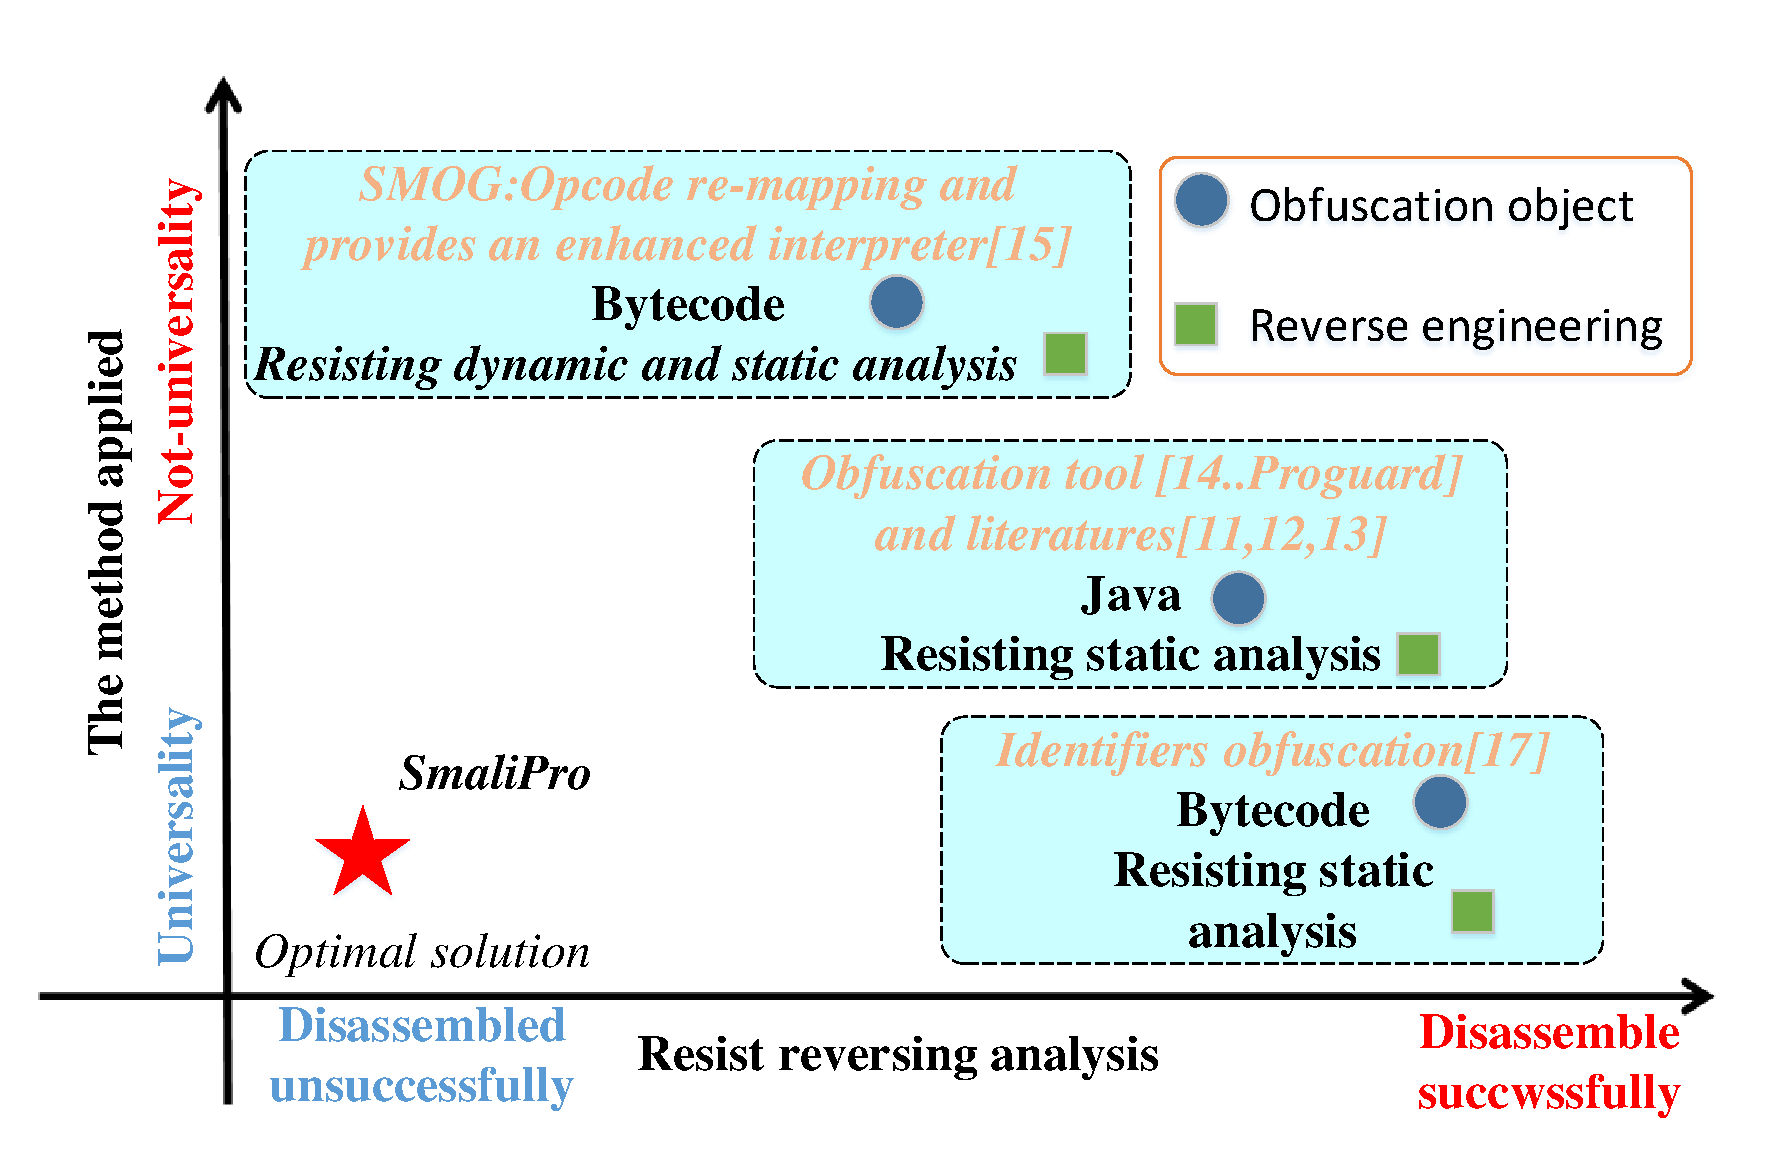
\includegraphics[width=0.8\columnwidth]{fig/fig1.pdf}\\
%  \caption{Design Space: comparing to related work.}\label{fig:Figure 1}
%  \FIXME{Change this into a table.}
%\end{figure}

%In this paper we propose SmaliPro, a comprehensive protection system based on obfuscated smali, an intuitive assembly language for Dalvik bytecode. Dalvik VM is one of the core part of the android mobile device platform and can support the form of .dex bytecode from Java source code. Its instructions are based on the architecture of register, so the constant pool was modified to use the index of 32 bits, which can simplify the interpreter. Therefore the constants and the return values of the function within smali code are stored in the 32-bit registers. When Dalvik VM performs the bytecode flow, it gets out the operand from the corresponding register in terms of the opcode, regardless of what the type of register is. According to this characteristic, we can confuse the data flow for the access procedure of register data, and combine opaque predicates\cite{13,17,18} technology to confuse the control flow. This method can resist decompiling and do not need the developer to provide the Java source code. The advantage of Our work is showing Figure\ref{fig:Figure 1}. We can see that the protection method will not only resist disassembled, but have universality.
%
%The core concept of SmaliPro is obfuscating the access procedure of constants in the registers. But the verifier component of Android runtime system(\emph{CodeVerify.app; DexVerify.cpp}) is referred to as VFY by Dalvik VM, which verifies the type of registers when loading the class. So our obfuscated application is not normally running. It is the challenge in this paper. In order to solve the problem, we use the dex dynamic loading technology and Dalvik runtime tampering technology, which is explained in Section 4.3.

In this paper, we present \ToolName, a novel bytecode level code obfuscation system for Android applications. \ToolName advances prior work in the following ways. Firstly, \ToolName performs code obfuscation on the bytecode level, so it does not require accessing to the source code and as a result the obfuscated code will not be optimized out by the compiler. Secondly, it obfuscates the dynamic program control flow when calling key protected functions. This significantly increases the difficulty for dynamic code analysis. \ToolName exploits two aspects of the Android Dex bytecode definition: (1) all except for floating operands are based on a 32-bit register and (2) the instruction follows a function call is always used to retrieve the return value of the function. Our approach utilizes the register structure of Dex to pack two 32-bit operands into a single 64-bit data item, so that any attempt in decoding the protected operands will receive incorrect information. We leverage the calling conversion of Dex, to insert opaque predicates (i.e. code with complex logic but does not get executed) between instructions of the function call and return value retrieval. Doing so not only makes it harder for the attacker to obtain the return value, but also obfuscates the dynamic program behavior.

We have evaluated our approach by using \ToolName to protect a number of
representative Android application operations. Experimental results show that
our approach can protect software against sophisticated reverse engineering
tools, including Jeb, Dex2Jar, dexdump and IDA pro, with less than
\FIXME{xx}\% increment in code size and runtime overhead.
This paper makes two specific contributions:
\begin{itemize}
\item It is the first work to exploit the register structure and calling convention of Android Dex for code protection;
\item It is the first byte-code level code obfuscation scheme that protects software against static and dynamic code analysis.

%\item This paper designs and implements a system SmaliPro based on smali code confusion, it does not need the developer to provide the Java source code and protects their intellectual property rights.
%\item SmaliPro aims at comprehensive protection of Android apps. It could resist not only static analysis but also dynamic analysis because the obfuscated bytecode cannot be correctly decompiled by the attacker.
%\item The performance overhead of obfuscated app is compared with the unprotected app, and the obfuscation method is evaluated by potency, resilience, availability and cost.
\end{itemize}

%\textbf{Structure of the paper:} We provide background and describe motivation in Section 2. Section 3 presents the overview of our system and Section 4 introduce the process of system implementation in detail. In Section 5, we discuss the potency, resilience and cost of the obfuscation method, and in Section 6 we deliberate evaluation of code obfuscation against current popular reverse tools and the overhead. Most relevant work in Android code obfuscation is discussed in Section7. Finally, the concluding remarks are given in Section 8. 